\chapter{Basic Procedure of MATSim and Other Equilibrium-based Transport Microsimulations}
\label{ch:basicprocedure}
% ##################################################################################################################
\hfill \textbf{Author:} Andreas Horni 

\begin{center} 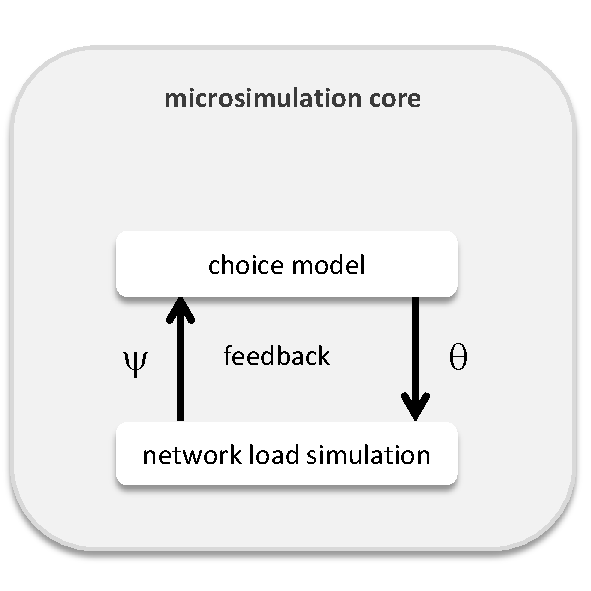
\includegraphics[width=0.3\textwidth, angle=0]{understanding/figures/fixedpoint.pdf} \end{center}

% ##################################################################################################################
The basic procedure of equilibrium-based microsimulations, such as MATSim or TRANSIMS is depicted in Figure \ref{fig:maxUtf}. A comprehensive (discrete) choice model is applied to a population for a specific choice situation. The choices are forwarded to a network load simulation (sometimes also called the physical simulation or mobility simulation). This network simulation takes into account constraints, such as network capacities. Generalized travel costs, calculated in the simulation, are fed back to the choice model. The choice model is also subject to constraints such as opening hours. The microsimulation is instantiated by census data for the population, travel surveys to estimate the models and infrastructure information to define the constraints. This instantiation or application is described for the MATSim Zürich scenario by  \citet[][]{HorniEtAl_TechRep_IVT_2011_a}. %In a very general sense, utility-based transport microsimulations do utility-maximization subject to constraints following the discrete choice methodology.

% ----------
\createfigure%
{Basic procedure of transport microsimulations}%
{Basic procedure of transport microsimulations}%
{\label{fig:maxUtf}}%
{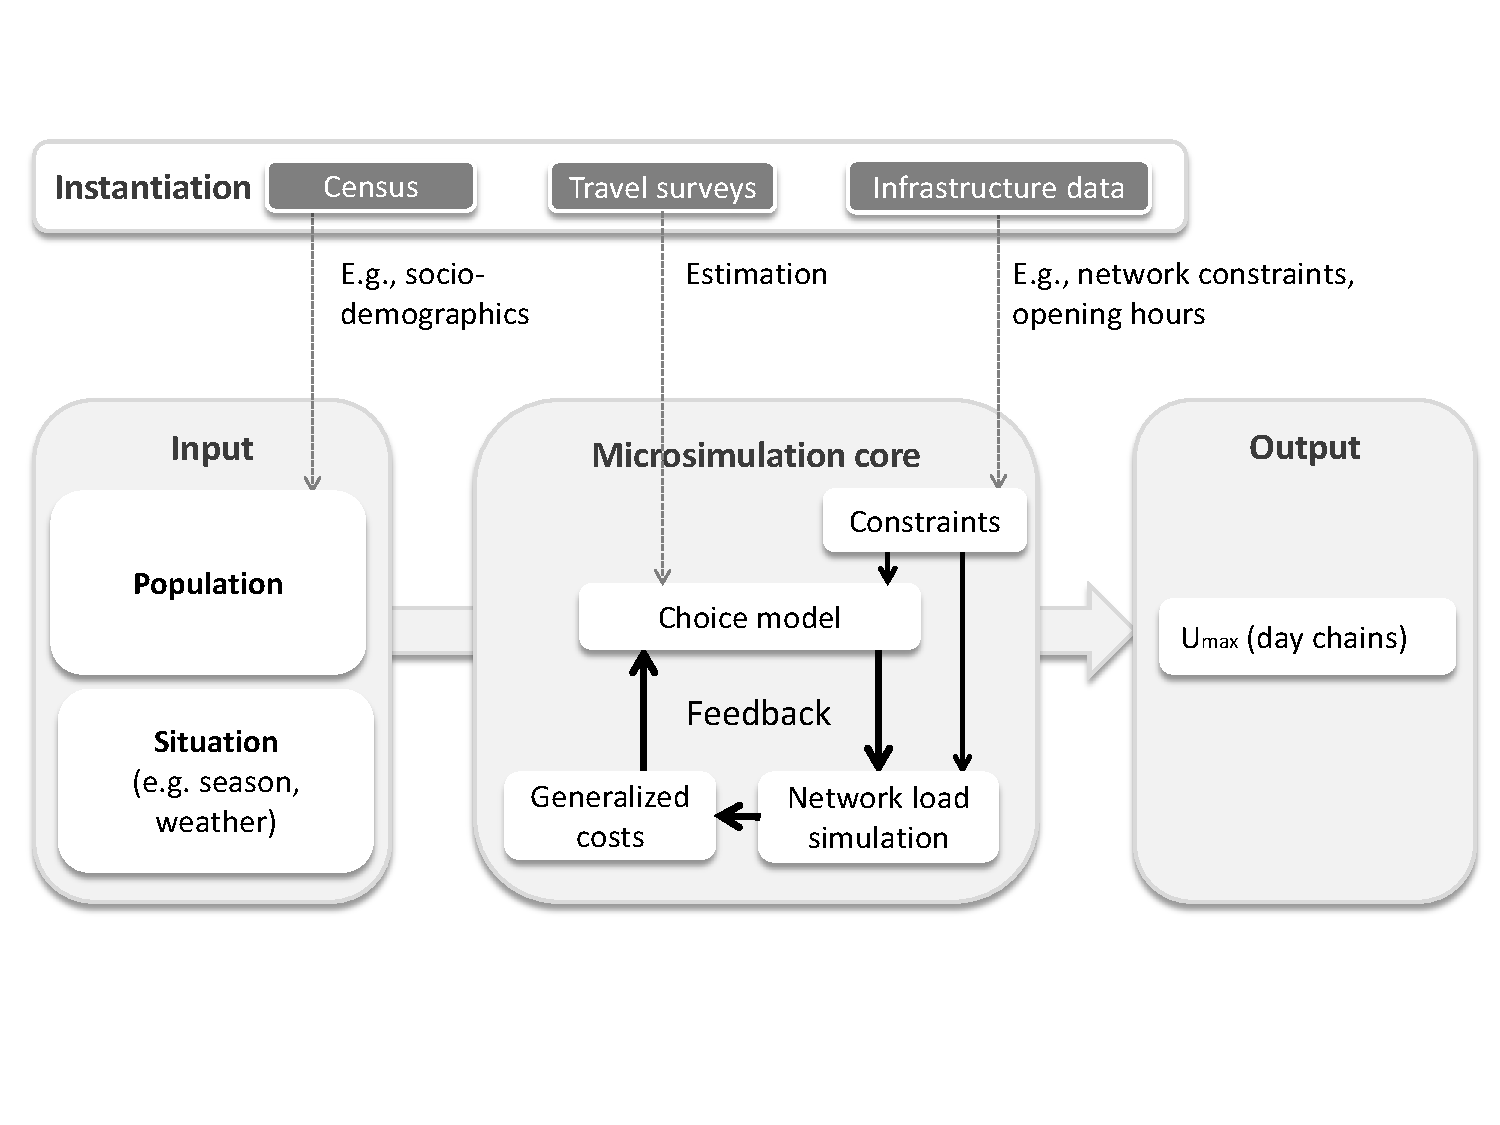
\includegraphics[width=0.99\textwidth, angle=0]{understanding/figures/maxUtf.pdf}}%
{}

% ----------

The cycle in the middle of Figure \ref{fig:maxUtf} represents a systematic relaxation process \citep[e.g.,][Figure 1.3]{Balmer_PhDThesis_2007}. In MATSim, the interpretation of the relaxation procedure is unclear. Sometimes the relaxation process is ascribed a behavioral interpretation, for example, day-to-day learning, where also the transition process and not only the final equilibrium has a meaning \citep[][p.128]{LiuEtAl_TransResA_2006}, \citep[][p.523]{NagelBarrett_IJMPC_1997}. An opposite perspective exists, where the relaxation procedure is just a numerical method to compute the Nash equilibrium without behavioral basis of the transitions.

To reveal similarities with known mathematical problems and their solution approaches a more abstract formulation can be established. 

The choice model draw is given as follows.
\begin{equation}
\label{eq:choiceModel}
\theta = h_0(\beta, y, \epsilon, \psi),
\end{equation}
where $\theta$ are the choices, $h_0$ is the choice model function, $\beta$ are the choice model coefficients, $\psi$ are the generalized costs given by the infrastructure conditions (e.g., network conditions), $y$ are further parameters such as the age of the decision maker and $\epsilon$ denotes the random error terms. 

Equilibrium-based transport microsimulations go beyond a single draw from a choice model. The parameters, such as the travel times, are an \emph{endogenous} component of these microsimulations. The circular relation between choices and the generalized costs can be written as a (usually non-linear) system of equations (see also Figure \ref{fig:fixedpoint}): 
\begin{equation}
\label{eq:initialSystem}
\begin{cases}
\theta = h_0(\beta, y, \epsilon, \psi) \\
\psi = h_1(\theta) 
\end{cases}
\end{equation}
where $\theta$ are the choices, $\psi$ are the generalized costs and $h_0$ and $h_1$ are mathematical maps. In microsimulations $h_0$ is implemented by the choice models and $h_1$ is the network loading simulation plus the succeeding conversion of infrastructure conditions into generalized costs. 

This can be rewritten as
\begin{equation}
\theta = h_0(\beta, y, \epsilon, h_1(\theta))
\end{equation}
%
or in a more general form:
%
\begin{equation}
\label{eq:phi}
\theta = \varphi(\theta, \beta, y, \epsilon) %f(\theta) = \varphi(\theta, \beta, y, \epsilon)
\end{equation}
%
%
% ----------
\createfigure%
{Fixed point problem}%
{Fixed point problem}%
{\label{fig:fixedpoint}}%
{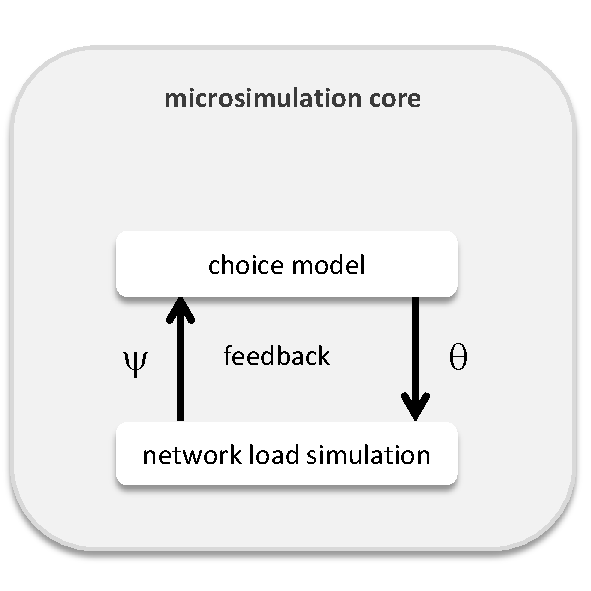
\includegraphics[width=0.4\textwidth, angle=0]{understanding/figures/fixedpoint.pdf}}%
{}
%
% ----------
%
This is a fixed point problem (see e.g., \citet[][p.6]{RamaduraiUkkusuri_TechRep_RPI_2008}, \citet[][]{BierlaireCrittin_TransScience_2006, KaufmanEtAl_TransResC_1998, RamaduraiUkkusuri_NSE_2010}). The fixed points are found by iteratively applying Equation \ref{eq:phi}. In the microsimulation context, \emph{iteratively}, the outcomes of the comprehensive choice model are directed to a network load simulation, whose outcomes (the infrastructure conditions) are in turn fed back to the choice model. But naively doing this most probably leads to very bad convergence behavior.

From numerics it is known that fixed point problems can be transformed such that convergence behavior is improved. This is explained with an example. In numerics root finding problems given as $f(x)=0$ are often transformed into fixed point problems as
\begin{equation}
\label{eq:fpf}
x=g(x)
\end{equation}
where the fixed points are the solutions of the root finding problem. As fixed point problems can be transformed, infinitely many possibilities exist for the choice of $g(.)$. For example the root finding problem $f(x)=x^2-2x-3=0$ can be transformed by using $g_0(x)=\sqrt{2x+3}$ or $g_1(x)=\frac{3}{x-2}$ or $g_2(x)=\frac{x^2-3}{2}$ to name a few. The choice of $g(.)$ thereby has a crucial impact on the convergence behavior, i.e., dependent on the form of $g(.)$ and the initial point $\theta_0$ the iterations may converge to a fixed point with different speed, are attracted by an orbit or may also move through the state space in a completely chaotic manner. In the example above, starting from $x_0=4$, $g_0(x)$ converges, $g_1(x)$ also converges but slower and $g_2(x)$ diverges. In numerics, the Picard method \citep[][p.2ff]{Vogt_TechRep_IfMath_2001} is improved by e.g., the Newton-Raphson method \citep[][p.28ff]{Vogt_TechRep_IfMath_2001}, which employs an efficient mapping for $g(.)$. 

A very similar approach is maybe productive for transport modeling; $\varphi(.)$ (which corresponds to $g(.)$) should be chosen reasonable, such that fixed points are found efficiently.

In first generation models, the fixed points are searched by implementing $\varphi(.)$ with iterative numerical algorithms such as the \emph{method of successive averages} (MSA) \citep[][p.342f]{OrtuzarWillumsen_2001} or the Frank-Wolfe algorithm \citep[][]{FrankWolfe_NRLQ_1956}, \citep[see also][p.4]{CorreaStier_Cochran_2010}. Every person searches its optimum subject to competition leading to an equilibrium state. This is achieved in the MSA by moving a certain share of the flow to the cheapest route, while taking it away from the remaining routes per OD-relation. For first generation models, much is known about existence, stability, uniqueness and computation of fixed points. Thus, by continuing the lines of the first generation models, one can hope to produce something reasonable also for second generation models, but this has to be investigated further. As shown in Section \ref{sec:co-ev}, a possible implementation of $\varphi(.)$ for MATSim is a co-evolutionary algorithm, which, in practice, has shown to efficiently lead to behaviorally sound fixed points.

% ##################################################################################################################